%% LaTeX-Beamer template for KIT design
%% by Erik Burger, Christian Hammer
%% title picture by Klaus Krogmann
%%
%% version 2.0
%%
%% mostly compatible to KIT corporate design v2.0
%% http://intranet.kit.edu/gestaltungsrichtlinien.php
%%
%% Problems, bugs and comments to
%% burger@kit.edu

\documentclass[18pt]{beamer}
\usetheme{kit}

%% TITLE PICTURE

% if a custom picture is to be used on the title page, copy it into the 'logos'
% directory, in the line below, replace 'mypicture' with the 
% filename (without extension) and uncomment the following line
% (picture proportions: 63 : 20, *.eps format if you use latex+dvips+ps2pdf,
% *.jpg/*.png/*.pdf if you use pdflatex)

%\titleimage{mypicture}

%% TITLE LOGO

% for a custom logo on the front page, copy your file into the 'logos'
% directory, insert the filename in the line below and uncomment it

%\titlelogo{mylogo}

% (*.eps format if you use latex+dvips+ps2pdf,
% *.jpg/*.png/*.pdf if you use pdflatex)

%% BIBTEX ICON/KEY

% if you want to see BibTeX keys in the references view instead of the symbol,
% uncomment the following line
% \usebibitemtemplate{\insertbiblabel}

% the presentation starts here

% change the following line to "ngerman" for German style date and logos
% change the following line to "english" for English style date and logos
\selectlanguage{ngerman}

\beamertemplatenavigationsymbolsempty

\usepackage{listings}
\definecolor{darkgray}{rgb}{0.95,0.95,0.95}
\definecolor{darkgreen}{rgb}{0.05,0.7,0.05}
\lstset{ language=Java,
	backgroundcolor=\color{darkgray}, 
	numbers=none, 
	keywordstyle=\color{black}\bfseries,
	tabsize=2,
	showspaces=false,               % show spaces adding particular underscores
	showstringspaces=false,         % underline spaces within strings
	showtabs=false, 
}



\title[Tutorium03]{Tutorium 03: Überschreiben und Überladen + Zustandsdiagramm}
\subtitle{Softwaretechnik im SS 2011, Tutorium 4}
\author{Jürgen Walter}
\date{\today}

\institute{Chair for Software Design and Quality}

\begin{document}

%title page
\begin{frame}
\titlepage
\end{frame}

%table of contents
\frame{
\frametitle{Was machen wir heute?}
	\tableofcontents
}

\section{Altes Übungsblatt}

\subsection{Altes Übungsblatt}
\frame {
\frametitle{Altes Übungsblatt}
	\begin{block}{Aufgabe 1: Sequenzdiagramm}
	\begin{itemize}
	\item Probleme mit Unterschied synchrone vs asynchrone Kommunikation
	\item Pfeilspitze ausmalen oder nicht?
	\end{itemize}
	\end{block}
}

\frame {
\frametitle{Altes Übungsblatt}
	\begin{block}{synchroner Nachrichten}
	\begin{itemize}
	\item Warten immer bis der aufgerufene fertig ist 
	\item (auch wenn keine Antworten gegeben werden)
	\end{itemize}
	\end{block}
	\pause

	\begin{block}{Antworten}
	\begin{itemize}
	\item nur bei synchronen Nachrichten möglich, optional
	\end{itemize}
	\end{block}
	\pause

	\begin{block}{asynchrone Nachrichten}
	\begin{itemize}
	\item "Mach es irgendwann zuende, ich bin nicht von dir abhängig!"
	\item z.B. Zerstörung eins Threads der nichts mehr tut, hier sollte das Programm nicht warten
	\item Entsprechen unsynchronisierten Thread-Operationen
	\item schneller, aber schwerer zu debuggen
	\end{itemize}
	\end{block}
}

\frame {
\frametitle{Altes Übungsblatt}
	\begin{block}{Sequenzdiagramm - Kommunikation}
	\begin{center}
	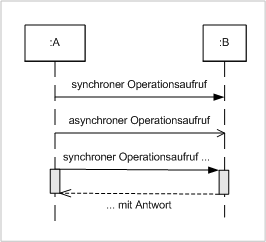
\includegraphics[width=0.6\textwidth]{pics/SequenzDiagramm1}
	\end{center}
	\end{block}
}

\frame {
\frametitle{Altes Übungsblatt}
	\begin{block}{Aufgabe 2: Zustandsdiagramm}
	\begin{itemize}
	\item Überwiegend richtig gelöst, sehr schön!
	\end{itemize}
	\end{block}
	\pause
	\begin{block}{Aufgabe 3:  Grafische Oberfläche für Floyd-Steinberg} 
	\begin{itemize}
	\item BLA BLA BLA
	\item BLA BLA BLA
	\item BLA BLA BLA
	\end{itemize}
	\end{block}
}

\subsection{Zum Aufwärmen ...}
\frame {
\frametitle{Wahr oder falsch?}
\begin{itemize}
	\color<2->[rgb]{1,0,0}
	\item Implementierungsvererbung ist die Voraussetzung für Signaturvererbung 
	\color[rgb]{0,0,0}
	\pause
	\color<3->[rgb]{0,1,0}
	\item Ein Modul ist eine Menge von Programmelementen, die nach dem Geheimnisprinzip gemeinsam entworfen und geändert werden.
	\color[rgb]{0,0,0}
	
	\pause
	\color<4->[rgb]{1,0,0}
	\item Wenn eine Benutzthierarchie nur transitive Zyklen aufweist, heißt sie Benutztrelation
	\color[rgb]{0,0,0}
	\pause
	\color<5->[rgb]{1,0,0}
	\item Software ist leichter zu ändern als ein physisches Produkt vergleichbarer Komplexität.
	\color[rgb]{0,0,0}
	\pause
	\color<6->[rgb]{1,0,0}
	\item In Java muss eine abstrakte Klasse, die eine Schnittstelle implementiert, alle in der Schnittstelle vorgegebenen Methoden implementieren
	\color[rgb]{0,0,0}

\end{itemize}
}

\section{Überladen und Überschreiben}
\subsection{Vererbung}

\frame{
\frametitle{Swing Tipps}
	\begin{block}{Layouts}
	\begin{itemize}
	\item um Swing Komponenten anzuordnen verwendet man Layouts \pause
	\item es gibt sehr viele Varianten: \url{http://download.oracle.com/javase/tutorial/uiswing/layout/visual.html}  \pause
	\item für ÜB3 habt ihr freie Wahl, daher bieten sich \texttt{FlowLayout} oder ein vertikales \texttt{BoxLayout} an 		\pause
	\item für bessere Strukturierung: gruppiert mehrere Komponenten mit einem JPanel  \pause
	\item jeder Swing Container kann sein eigenes Layout haben \pause
	\item default: JFrame - \texttt{BorderLayout}, JPanel -  \texttt{FlowLayout})
	\end{itemize}
	\end{block}
}
\begin{frame}[fragile]
\frametitle{Swing Tipps}
\begin{block}{Bilder anzeigen}
\begin{itemize}
\item grundsätzlich kann man auf jede Swing Komponente malen \pause
\item am einfachsten: \texttt{Icon} setzen \\
\url{http://download.oracle.com/javase/tutorial/uiswing/components/icon.html}  \pause
\end{itemize}
\end{block}

\begin{block}{Beispiel}
\begin{lstlisting}
	JFrame f = new JFrame();
	f.setDefaultCloseOperation(JFrame.EXIT_ON_CLOSE);
	f.add(new JLabel(new ImageIcon(image)));
	f.setSize(200,200);
	f.setVisible(true);
\end{lstlisting}
\end{block}
\end{frame}

\begin{frame}[fragile]
\frametitle{Swing Tipps}
\begin{block}{Beispiel}
\begin{lstlisting}
	JFrame f  = new JFrame();
	f.setDefaultCloseOperation(JFrame.EXIT_ON_CLOSE);
	f.setLayout(new FlowLayout());
	f.setSize(220,325);

	for (int i=0; i<20; i++) {
	  	f.add(new JLabel("Text"));
	  	f.add(new JButton("Button"));
	}
	f.setVisible(true);
\end{lstlisting}
\end{block}
\end{frame}

\subsection{Eclipse}
\frame {
\frametitle{Parameter in Eclipse übergeben}
	\begin{exampleblock}{Parameter übergeben I}
	\begin{center}
	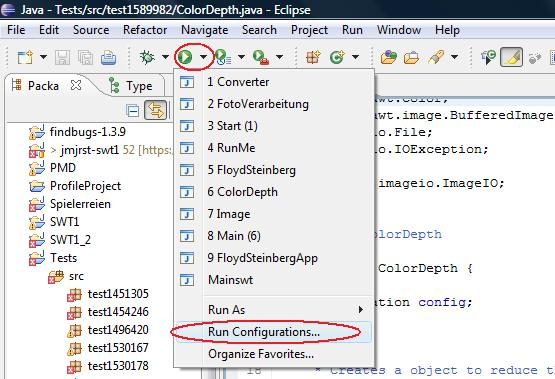
\includegraphics[scale=0.6]{pics/ParameterPassing1.jpg}
	\end{center}
	\end{exampleblock}
}

\frame {
\frametitle{Parameter in Eclipse übergeben}
	\begin{exampleblock}{Parameter übergeben II}
	\begin{center}
	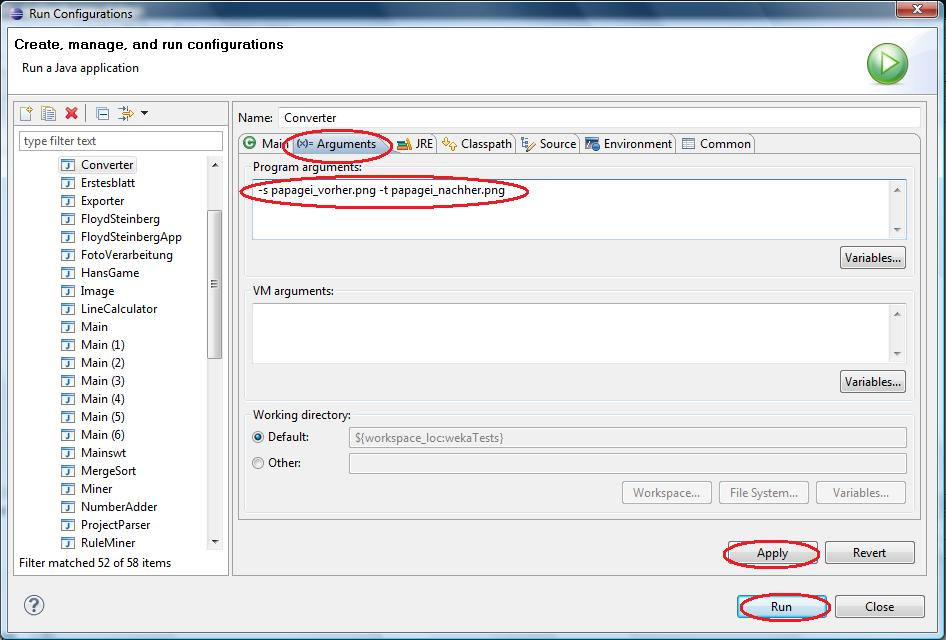
\includegraphics[scale=0.36]{pics/ParameterPassing2.jpg}
	\end{center}
	\end{exampleblock}
}

\section{UML}
\subsection{Zustandsdiagramm}

\frame{
\frametitle {Zustandsdiagramm} 
	\begin{itemize}
	\item Beschreibt mögliche Zustände eines Objekts sowie mögliche Zustandsübergänge
	\item Der Zustandsübergang (Transition) wird durch ein Ereignis ausgelöst
	\begin{center}
	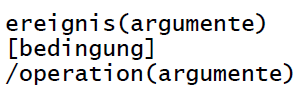
\includegraphics[scale=0.5]{pics/zustandsuebergang.png}
	\end{center}
	\item Zustandsübergang findet nur statt, wenn die Bedingung zu diesem Zeitpunkt erfüllt ist
	\item $\epsilon$ -Übergänge sind erlaubt
\end{itemize}
}

\frame {
\begin{exampleblock}{Beispiel Zustandsdiagramm}
\begin{center}
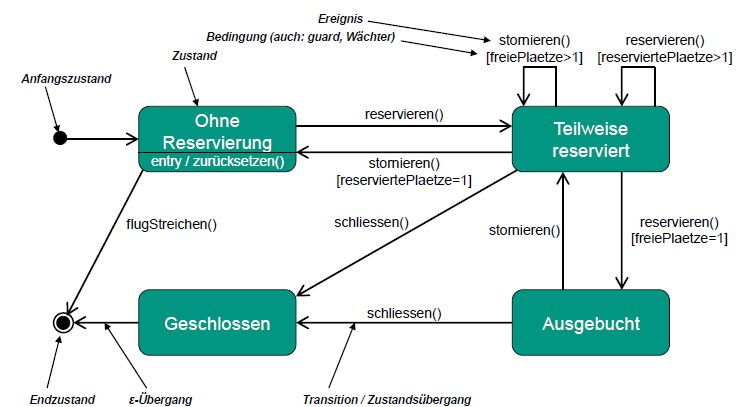
\includegraphics[scale=0.6]{pics/zustandsdiagramm.png}
\end{center}
\end{exampleblock}
}

\frame {
\begin{exampleblock}{Beispiel Zustandsdiagramm mit Gedächtnis}
\begin{center}
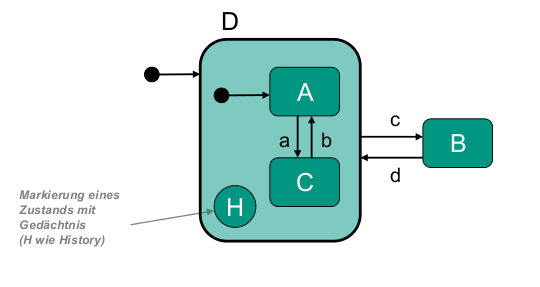
\includegraphics[scale=0.6]{pics/ZustandsDiagrammGedaechtnis.png}
\end{center}
\end{exampleblock}
}


\frame{
\frametitle {Zustandsdiagramm Aufgabe Klausur 2009 (1P)}
Gegeben ist der folgende UML-Zustandsautomat. Geben Sie an, in welcher Zustandskombination
sich der Zustandsautomat, jeweils ausgehend vom Startzustand, nach den beiden Eingabefolgen
befindet. 

\begin{center}
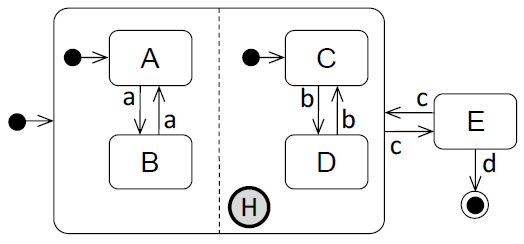
\includegraphics[scale=0.6]{pics/03/zustandN.png}
\end{center}
}

\frame{
\frametitle {Zustandsdiagramm Aufgabe Klausur 2009 5P)}
Wandeln Sie den UML-Zustandsautomaten in einen äquivalenten neuen um, der weder nebenläufige noch hierarchische Zustände oder Zustände mit Historie enthält. Leiten Sie die Namen für die Zustände wie folgt aus den Namen der Zustände des alten Automaten ab:
Regel 1: Die Kombination der alten Zustände 1 und 2 wird zum neuen Zustand $1 \times 2$.
Regel 2: Wurde der alte Zustand 1 vom alten Zustand 2 aus erreicht, ergibt dies den neuen
Zustand 1(2). 

\begin{center}
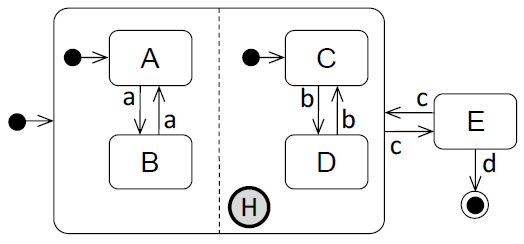
\includegraphics[scale=0.55]{pics/03/zustandN.png}
\end{center}
}

\frame {
\frametitle {Musterlösung} 
\begin{center}
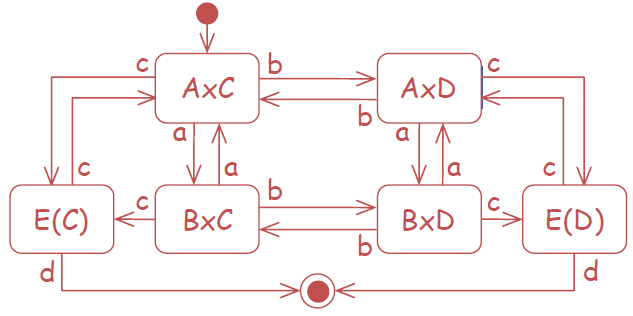
\includegraphics[scale=0.6]{pics/03/zustandNM.png}
\end{center}
}

\subsection{Sequenzdiagramm}

\frame {
	\frametitle {Sequenzdiagramm}
	\begin{block}{Sequenzdiagramm - Weiteres Beispiel}
	\begin{center}
	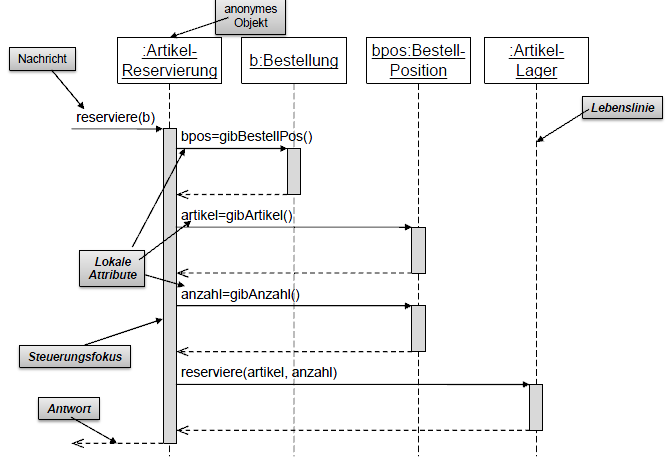
\includegraphics[width=0.8\textwidth]{pics/sequenzdiagrammBeispiel2.png}
	\end{center}
	\end{block}
}

%
%\frame {
%\frametitle {Aufgabe Sequenzdiagramm 2010 (5P)}
%\small {
%Ein Passagierjet p meldet seinen momentanen Kurs $k_p$ an den Kontrollturm. Der Kontrollturm beauftragt den nächsten freien Fluglotsen f zu berechnen, ob irgendwelche Flugobjekte ausweichen müssen. Der Fluglotse kommt zu dem Ergebnis, dass keine Kollisionsgefahr besteht und alle Flugobjekte ihren Kurs beibehalten können. Folglich antwortet er mit einem leeren Feld von Kursen. Anschließend meldet ein Helikopter h seinen Kurs $k_h$ an den Kontrollturm. Wieder ist der nächste verfügbare Fluglotse der Flug-lotse f. Dieser berechnet unter Berücksichtigung von $k_h$, ob nun Flugobjekte ausweichen müssen. Diesmal besteht eine Kollisionsgefahr zwischen dem Passagierjet und dem Helikopter. Deswegen antwortet der Fluglotse mit zwei Ausweichkursen $k’_p$ und $k’_h$ für den Passagierjet bzw. den Helikopter. Der Kontrollturm weist daraufhin den Passagierjet und den Helikopter an ihre Kurse auf den jeweiligen Ausweichkurs zu ändern.
%\\
%Hinweis: Modellieren Sie die Kurse nicht als Objekte mit Lebenslinie. Wenn Sie Kurse als Parameter/Rückgabewert benötigen, verwenden Sie die vorgegebenen Bezeichner aus dem Szenario. Zeichnen Sie zu jedem Methodenaufruf auch die Rückantwort ein
%}
%}
%
%\frame {
%\frametitle {Musterlösung} 
%\begin{center}
%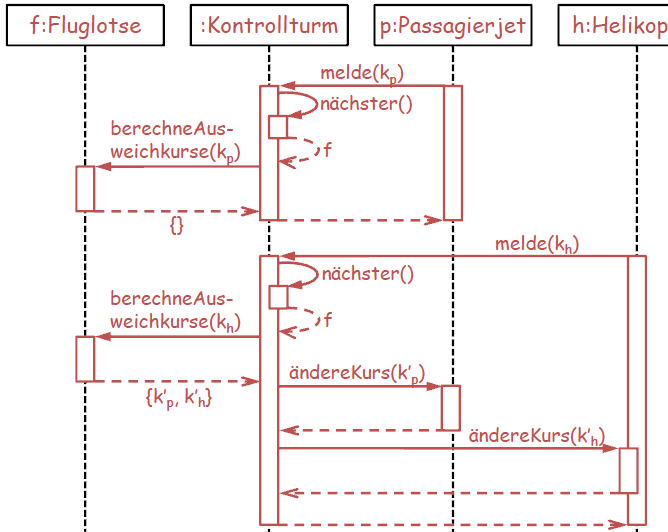
\includegraphics[scale=0.5]{pics/MSequenzdiagrammAufgabe.png}
%\end{center}
%}

\section{Ende}

\subsection{Tipps zum nächsten Übungsblatt}

\frame{
\frametitle{Tipps zum nächsten Übungsblatt}

\begin{block}{Aufgabe 1 - UML Zustandautomaten}
\begin{itemize}
\item a) Umkehrung der Klausuraufgabe des letzten Tutoriums
\item b) Das History H gilt nur für den rechten Abschnitt
\end{itemize}
\end{block}

\begin{block}{Aufgabe 2 - Überladen und Überschreiben}
\begin{itemize} \pause
\item Vererbung ist das grundlegende Konzept der objektorientierten Programmierung
\item Hier könnt ihr relativ schnell merken, ob ihr es verstanden habt!
\end{itemize}
\end{block}
}


\frame{
\frametitle{Tipps zum nächsten Übungsblatt}
\begin{block}{Aufgabe 3 - Programmieren}
\begin{itemize}
\item Einfügen des der letzten Programmieraufgabe in JMRST
\item TODO Wo muss ich was einfügen
\item Wichtig: Sprache muss in eine Property Datei ausgelagert werden
% \url{http://download.oracle.com/javase/tutorial/uiswing/layout/visual.html}
\end{itemize}
\end{block}
}

\frame{
\frametitle{Tipps zum nächsten Übungsblatt}
\begin{block}{Bonusaufgabe - Kammerjäger}
\begin{itemize}
\item Für die, die sich nicht ausgelastet fühlen
\item Viel Aufwand für 3 Punkte
\item Nutzt Eclipse tools zum profilen
\end{itemize}
\end{block}
}


\frame{
\frametitle{Bis zum nächsten Mal}
	\begin{center}
	
\includegraphics[height=200pt]{pics/02_zeitmaschine}
	\end{center}
}


\end{document}
